\documentclass[aspectratio=169]{beamer}
\usepackage{graphicx}
\usepackage{listings}
\usepackage{hyperref}

\usetheme{metropolis}
\title{git/GitHub for Developers}
\institute{Engineers for Exploration, UC San Diego}
\setbeamertemplate{caption}[numbered]
\lstset{
    basicstyle=\ttfamily
}
\logo{
\includegraphics[height=.65cm,keepaspectratio]{e4e_logo_350x136.png}}
\begin{document}
\maketitle
\begin{frame}{Introduction}
    \begin{itemize}
        \item \textbf{Git vs. GitHub:} Distributed VCS vs. collaboration platform.
        \item \textbf{Purpose:} Enhances project management and teamwork.
    \end{itemize}
    \begin{center}
        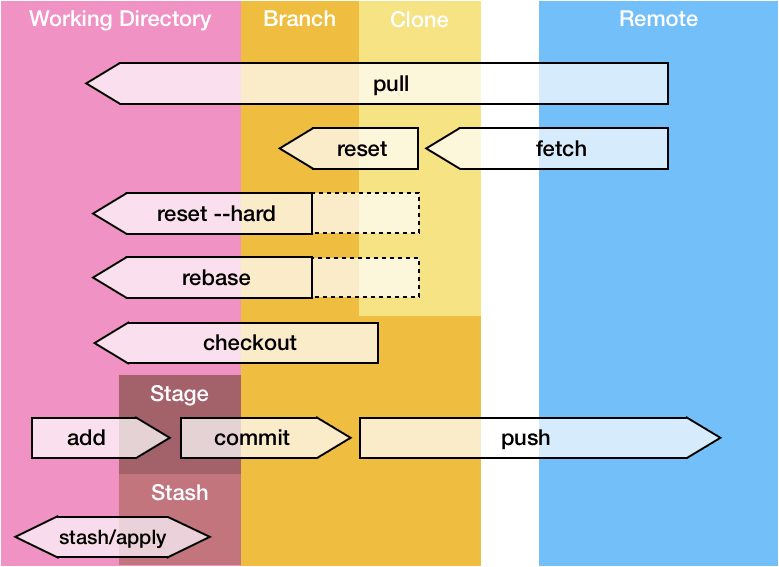
\includegraphics[scale=.25]{git_commands.png}
    \end{center}
\end{frame}
\begin{frame}{Git Workflows}
    \begin{itemize}
        \item Feature Branch Workflow
        \item Gitflow Workflow
        \item Fork Workflow
    \end{itemize}
\end{frame}
\begin{frame}{Feature Branch Workflow}
    \begin{itemize}
        \item Develop each feature in its own branch.
        \item Merges via pull requests for code review.
        \item Keeps main branch stable, encourages collaboration.
        \item Ideal for projects with simultaneous feature development.
    \end{itemize}
    \begin{center}
        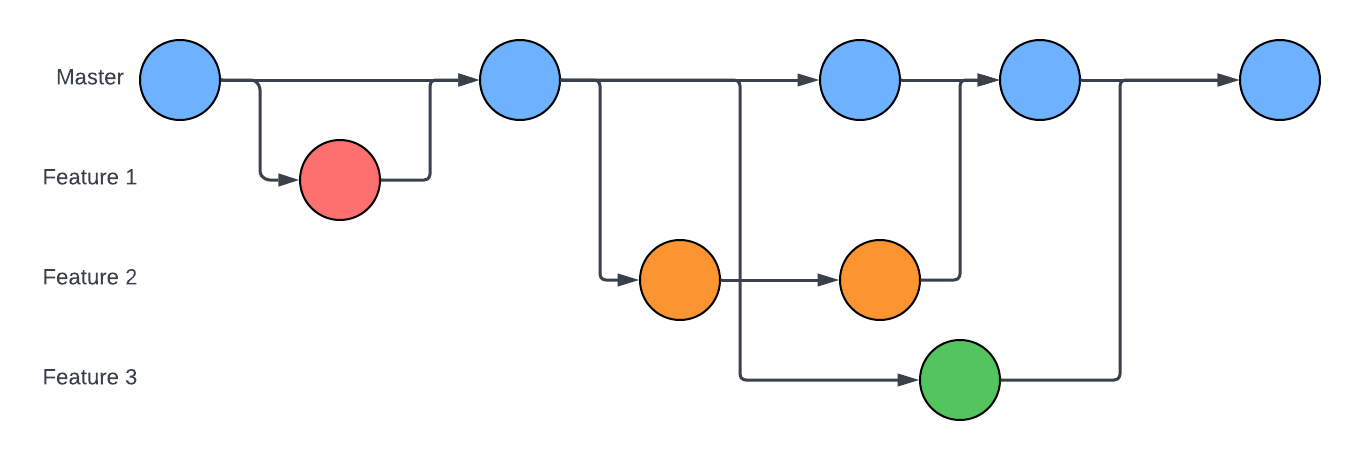
\includegraphics[scale=.25]{feature_workflow_diagram.png}
    \end{center}
\end{frame}
\begin{frame}{Gitflow Workflow}
    \begin{itemize}
        \item Structured model: development, features, releases, hotfixes.
        \item Systematic release management, clear branch roles.
        \item Tracks progress efficiently, supports parallel releases.
        \item Suited for scheduled release cycles.
    \end{itemize}
    \begin{center}
        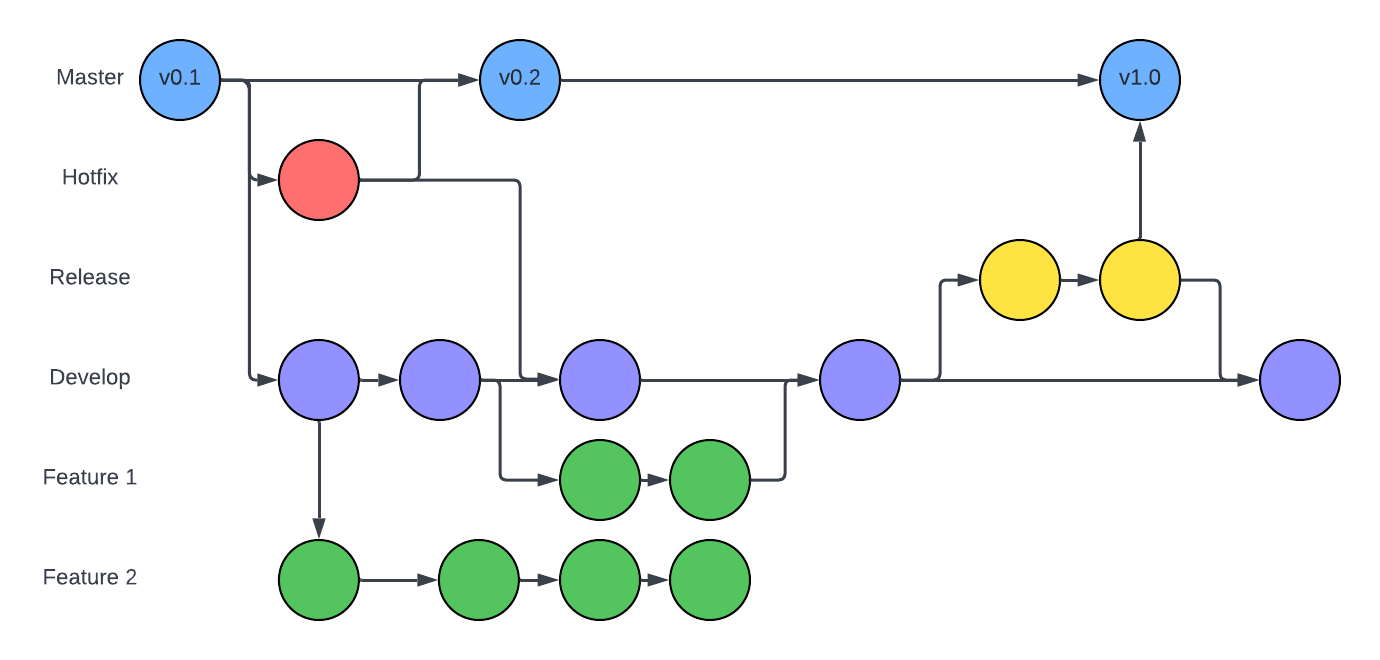
\includegraphics[scale=.2]{gitflow_workflow_diagram.png}
    \end{center}
\end{frame}
\begin{frame}{Fork Workflow}
    \begin{itemize}
        \item Developers work on personal repository copies.
        \item Changes proposed via pull requests.
        \item Encourages external contributions, safe experimentation.
        \item Ideal for open-source and large collaborations.
    \end{itemize}
    \begin{center}
        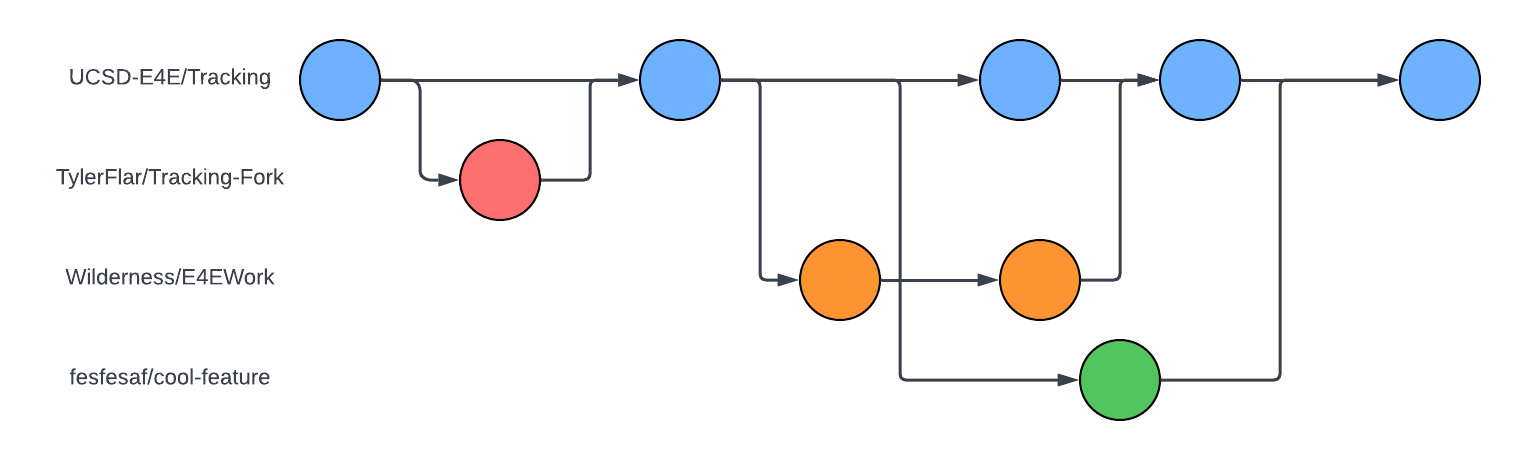
\includegraphics[scale=.25]{fork_workflow_diagram.png}
    \end{center}
\end{frame}
\begin{frame}{Tags}
    \begin{itemize}
        \item Marks significant project milestones.
        \item Useful for release points, use semantic versioning.
        \item Lightweight tags: \textit{git tag tagname}.
        \item Annotated tags: \textit{git tag -a tagname ``message''}.
        \item List/delete tags: \textit{git tag}, \textit{git tag -d tagname}.
    \end{itemize}
\end{frame}    
\begin{frame}{Pull Requests (PR) Management}
    \begin{itemize}
        \item Keep PRs small for easy review.
        \item Use checklists for consistent reviews.
        \item Automate tests and checks via GitHub Actions.
    \end{itemize}
\end{frame}
\begin{frame}{Releases}
    \begin{itemize}
        \item Draft new release, choose git tag.
        \item Add release notes describing changes.
        \item Bundles code, executables, and assets.
        \item Detailed notes inform users of updates.
        \item Example: https://github.com/HumanSignal/label-studio/releases
    \end{itemize}
\end{frame}
\begin{frame}{GitHub Actions for Automation}
    \begin{itemize}
        \item Triggered by GitHub events (push, PRs).
        \item Workflows combine actions in YAML files.
        \item Runs on GitHub-hosted or self-hosted runners.
        \item Automates tests and deployment on PR merge.
        \item Auto-assigns issues, auto-labels PRs by path.
    \end{itemize}
\end{frame}
\begin{frame}{Putting it Together}
    \begin{itemize}
        \item Combine Tags, Releases, and GitHub Actions.
        \item Interact with source code.
        \item Example: https://github.com/TylerFlar/MinecraftDiscord-CrossChat
    \end{itemize}
\end{frame}
\begin{frame}{Securing Your Project}
    \begin{itemize}
        \item Set branch protection rules for safety.
        \item Dependabot scans and fixes vulnerabilities.
        \item Secret scanning detects exposed credentials.
        \item Code scanning for vulnerabilities on push.
    \end{itemize}
    \begin{center}
        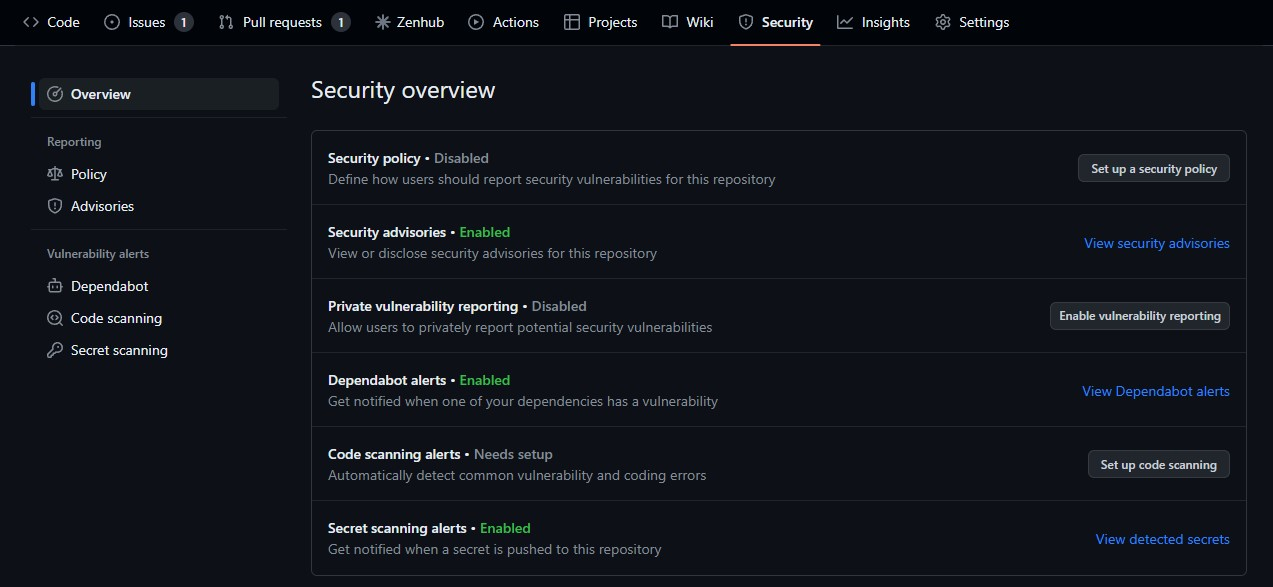
\includegraphics[scale=.5]{github_security.jpg}
    \end{center}
\end{frame}
\begin{frame}{Extras: Advanced Git}
    \begin{itemize}
        \item Interactive Rebase*: Rewrite history, edit commits.
        \item Stashing*: Temporarily shelf changes for tasks.
        \item Cherry-picking: Apply commit to another branch.
        \item * Not recommended for shared/remote repositories.
    \end{itemize}
\end{frame}
\begin{frame}{Cherry-picking}
    \begin{itemize}
        \item \textit{git cherry-pick commit-hash}
    \end{itemize}
    \begin{center}
        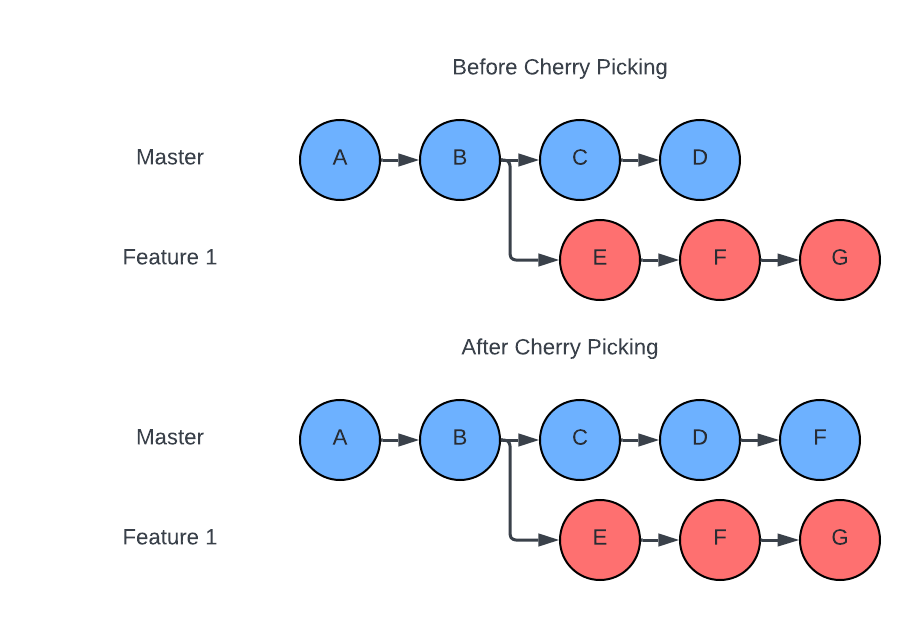
\includegraphics[scale=.25]{cherry_diagram.png}
    \end{center}
\end{frame}
\end{document}